\section{Training Approach}

\begin{outline}
  Describe the reinforcement learning or supervised learning approach
  used to train the CNN models.
\end{outline}

Below is the equation used as the input to the contact model
(\autoref{fig:data-training-model-data-comparison}).

\[
  \mathbf{x} =
  \begin{bmatrix}
    \mathbf p_{b,xy} \\
    \mathbf r_{w,z} \\
    \mathbf v_b \\
    \mathbf \omega_b \\
    \mathbf u
  \end{bmatrix}
\]

where
$\mathbf p_{b,xy}$ is the $x$ and $y$ position all end effectors in
the base frame as a single vector,
$\mathbf r_{w,z}$ is the height of the robot's COM in the world frame.

The model is trained on $y$, the heuristically calculated footstep
cost maps (\autoref{fig:data-footstep-cost-map}).

Here, the inclusion of $\mathbf \omega_b$ differs from
\cite{bratta_contactnet_2024}

\begin{figure}
  \centering
  \begin{minipage}[T]{0.45\textwidth}
    \centering
    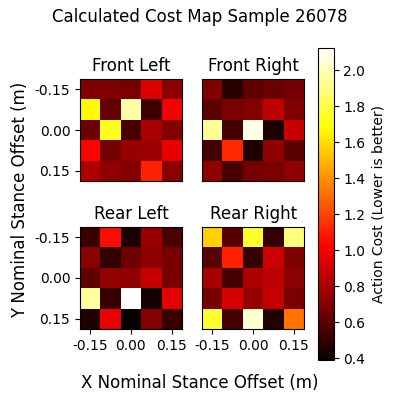
\includegraphics[width=\textwidth]{images/data/training/calculated-quadruped_2025-09-19T08-16-04.png}
  \end{minipage}
  \hfill
  \begin{minipage}[T]{0.45\textwidth}
    \centering
    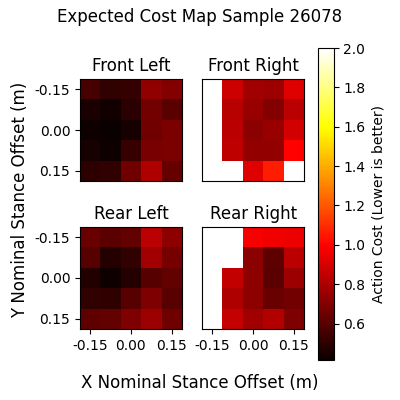
\includegraphics[width=\textwidth]{images/data/training/expected-quadruped_2025-09-19T08-16-04.png}
  \end{minipage}
  \hfill

  \caption{Training data samples showing calculated (left) and
  expected (right) quadruped images.}
  \label{fig:data-training-model-data-comparison}
\end{figure}

As in \cite{bratta_contactnet_2024}, the cost maps are normalized
to improve training performance.

\begin{figure}
  \centering
  \begin{minipage}[T]{0.45\textwidth}
    \centering
    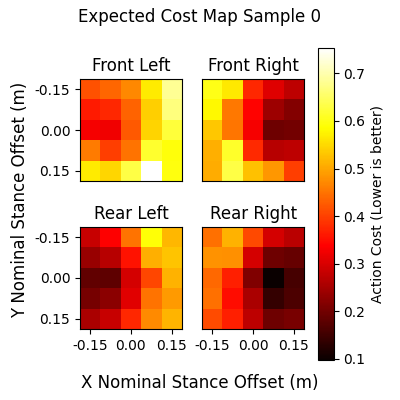
\includegraphics[width=\textwidth]{images/data/cost-map-normalization/un-normalized.png}
  \end{minipage}
  \hfill
  \begin{minipage}[T]{0.45\textwidth}
    \centering
    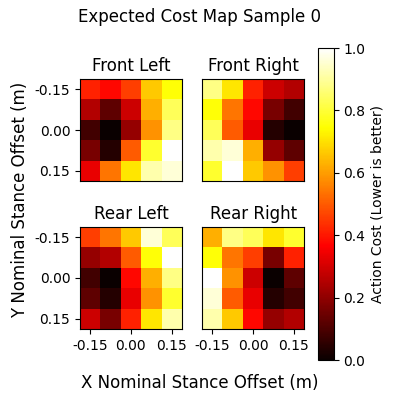
\includegraphics[width=\textwidth]{images/data/cost-map-normalization/normalized.png}
  \end{minipage}
  \hfill

  \caption{Cost map normalization showing un-normalized (left) and
  normalized (right) cost maps.}
  \label{fig:data-cost-map-normalization}
\end{figure}
